% arara: pdflatex: {shell: yes, synctex: yes, options: "-file-line-error-style"}
% arara: bibtex if found('log', 'undefined references')
% arara: pdflatex: {shell: yes, synctex: yes, options: "-file-line-error-style"}
% arara: pdflatex: {shell: yes, synctex: yes, options: "-file-line-error-style"}



% Before start, check the file README.txt
\documentclass[10pt,a4paper,twocolumn,english]{article}
\usepackage{sbsr}

%%%% This file presents the global settings for the document in LaTeX %%%%
%%%% (MORE INFORMATION IN README.txt) %%%%
%%%  The paper information must be declared below as well as its authors and affiliations %%%%

\title{Exploratory analysis of Recurrent deforestation warnings in 
São Félix do Xingu - Brazilian Amazon}

\author{Alber Sánchez Ipia$^1$, Guilherme Mataveli$^1$, Aline Pontes-Lopes$^1$ 
Sulimar Munira Caparoci Nogueira$^2$, and Luiz Aragão$^1$}

\address{$^1$Earth Observation and Geoinformatics Division - DIOTG, National 
Institute for Space Research - INPE, Av. dos Astronautas, 1758 - São José dos 
Campos - SP - Brazil alber.ipia@inpe.br, guilherme.mataveli@inpe.br, 
aline.lopes@inpe.br, luiz.aragao@inpe.br;
$^2$IDGeo - Inteligência Agrícola, suli.nogueira@gmail.com}

%%%% Beginning of the document %%%%

\begin{document}


% create the title %%%% (DO NOT CHANGE) %%%%
\twocolumn[
\begin{@twocolumnfalse}
\maketitle
\end{@twocolumnfalse}
]


%%%% Add each section file %%%%
%%%% (ALTER ONLY IF SECTIONS ARE INTRODUCED/REMOVED) %%%%

\section*{\textit {Abstract}} %%%% (DO NOT CHANGE) %%%%

\hspace{-1.5mm}\textit{ %%%% (DO NOT CHANGE) %%%%
%%%% Add the abstract below %%%%
%The abstract should appear at the top of the left-hand column of the text. The abstract should contain about 100 to 150 words. All manuscripts must be written in Portuguese, English or Spanish. Manuscripts must have a maximum of 4 pages including references.
Identifying forest degradation is as import as identifying deforestation, but 
even more challenging.
Due to the role of tropical forests in the Earth System, it is imperative to 
discover new ways to improve and characterize our knowledge about 
forest degradation.
This includes finding alternative uses for already existing data such as the 
warnings issued by the DETER system.
In this paper, we explore the DETER warnings in \textit{São Félix 
do Xingu} from 2016 to 2021 and compute their frequency over the same areas.
We found forest areas with up to 4 warnings 4 years apart and their mean time
between the first and second warnings is two years and one year between the 
second and the third.
Our results are important because they point to DETER as a source of data for 
analyzing the development of deforestation by recurrent degradation.
}
\\

%%%% Add the Key words below %%%%
\textit{\textbf{Key words --} %%%% (DO NOT CHANGE) %%%%
Degradation, Deforestation, DETER. %%%% (ADD KEY WORDS) %%%%
}



\section{Introduction}

% Background, known information.
The Amazon rainforest plays many roles in controlling the climate and avoiding the current climate crisis.
Not only it is home to countless species, but also regulates both the water and carbon cycles.
Besides, it is a massive carbon reservoir, and it is one of the potential tipping points at which poor management could trigger catastrophic and irreversible
changes to the climate system.

% Knowledge gap, unknown information.
The current advances in Ecology, Remote Sensing, and Computer Science have enabled the development of regional, continental and global deforestation monitoring systems (e.g., DETER, MapBiomas, Global Forest Watch).
However, detecting and monitoring forest degradation remains more challenging than detecting deforestation~\cite{Lambin:1999,Mitchell2017}.


% Hypothesis, question, purpose statement.
Given the importance of this issue, in this paper we present the spatial distribution of recurrent forest degradation in the Brazilian Amazon, which could help address the challenges in detecting it. 
We think that deforestation real-time forest monitoring systems, such as DETER that continuously issues deforestation alerts, inadvertently captures forest degradation processes at various stages.
% Approach, plan of attack, proposed solution.
The findings presented here are the results of processing 5 years of DETER 
alerts.

This paper extends the findings introduced in ~\cite{sanchez2023}.


\section{Material e methods}

For our analysis, we employed DETER data from August 2016 to July 2021. 
DETER is a real-time deforestation detection system developed by the National Institute of Space Research that is at the forefront of Brazil's efforts to control deforestation.
DETER has produced fast assessments of forest degradation and deforestation in the Brazilian Amazon since 2004~\cite{shimabukuro2006}. 
%TODO: Add statistics about DETER's dataset.

DETER mainly uses remote sensing imagery from the WFI camera on board of the CBERS satellites, producing alerts  of at least 3 ha which are tagged as wildfire scar, mining, deforestation with either exposed soil or vegetation, degradation, and selective cut with either disordered or geometric pattern~\cite{diniz2015a,f.g.assis2019}. 

Degradation and deforestation spots are identified by human experts on images enhanced with a color composition (red, near-infrared, and green) and a Linear Mixture Model~\cite{shimabukuro1991} (soil fraction) and the criteria of tone, color, shape, texture, and context. 
These experts draw DETER warnings (polygons) on top of a computer screen fix on a scale 1:100,000 using as background the latest primary forest polygon mask and previous DETER warnings~\cite{dealmeida2022}.
DETER data is publicly available at the TerraBrasilis portal~\cite{f.g.assis2019}. 

After downloading, we self-intersected the data (union operation) and re-projected them to the coordinate reference system UTM 22s.
We also removed duplicated vertices and enforced the right-hand rule for polygons.
Then we fixed geometry errors, and finally we removed alerts smaller than 3~ha.
This processing was applied using QGIS version 3.38.0~\cite{QGIS_software}.
We also computed the alerts' warning year using the PRODES calendar, which is the period from August to July; each PRODES year takes the year number from the last month of its period (July).

DETER alerts don't spatially match over time.
This means that it is only possible to match alert subareas consistently along the time dimension.
This is the reason for the data self-intersection mentioned above.
The \textit{subareas} resulting from this self-intersection correspond to polygons on which DETER alerts were issued on different dates, and are the base on which our analysis is founded.

Our analyses were carried out using the GNU's R language and environment for statistical computing and graphics to estimate statistics analysis~\cite{ihaka1996}.
Our source code is available online.~\footnote{R code available at \url{https://github.com/albhasan/treesburnareas}}

	
\section{Results}

DETER data show an abrupt fall in during PRODES year 2019 followed by an increasing trend in the area covered by its alerts. It is worth noticing that the distribution by area in homogenous for each year, particularly for 2021 (see ~Figure~\ref{fig:deter_warnings_area_size}).

\begin{figure}[h] 
    \begin{center}
    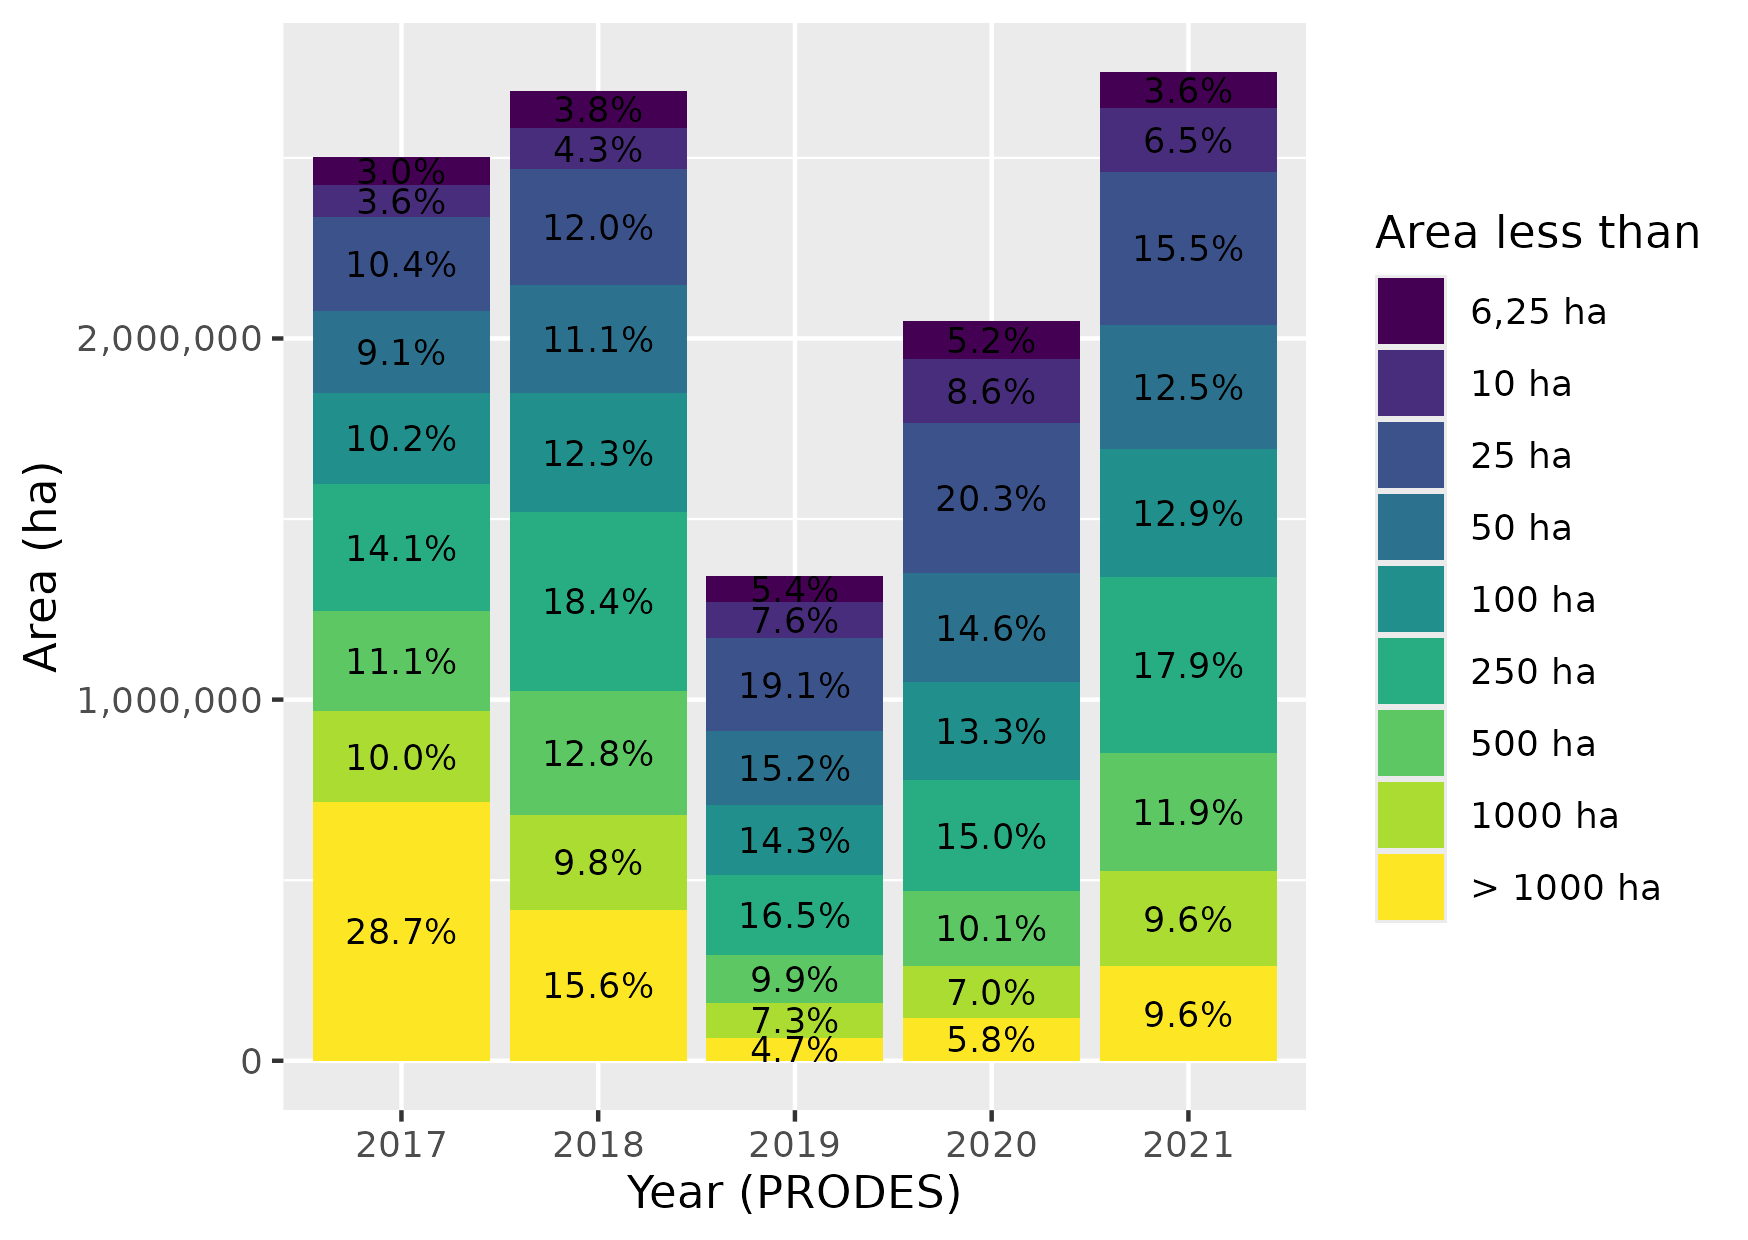
\includegraphics[width=\linewidth]{deter_warnings_area_size.png}
    \caption{Area of DETER alerts by year and size. The area covered by alerts
        peaked in 2018 and 2021. Note the increasing trend since 2019 and how
        their area distribution is relatively homogeneous along in 2021.}
    \label{fig:deter_warnings_area_size}
    \end{center}
\end{figure}

Moreover, the number of DETER alerts during the same period shows a somewhat similar pattern, characterized by the fact that half of yearly DETER alerts are issued for small areas (Figure~\ref{fig:deter_warnings_size}).

\begin{figure}[h] 
    \begin{center}
    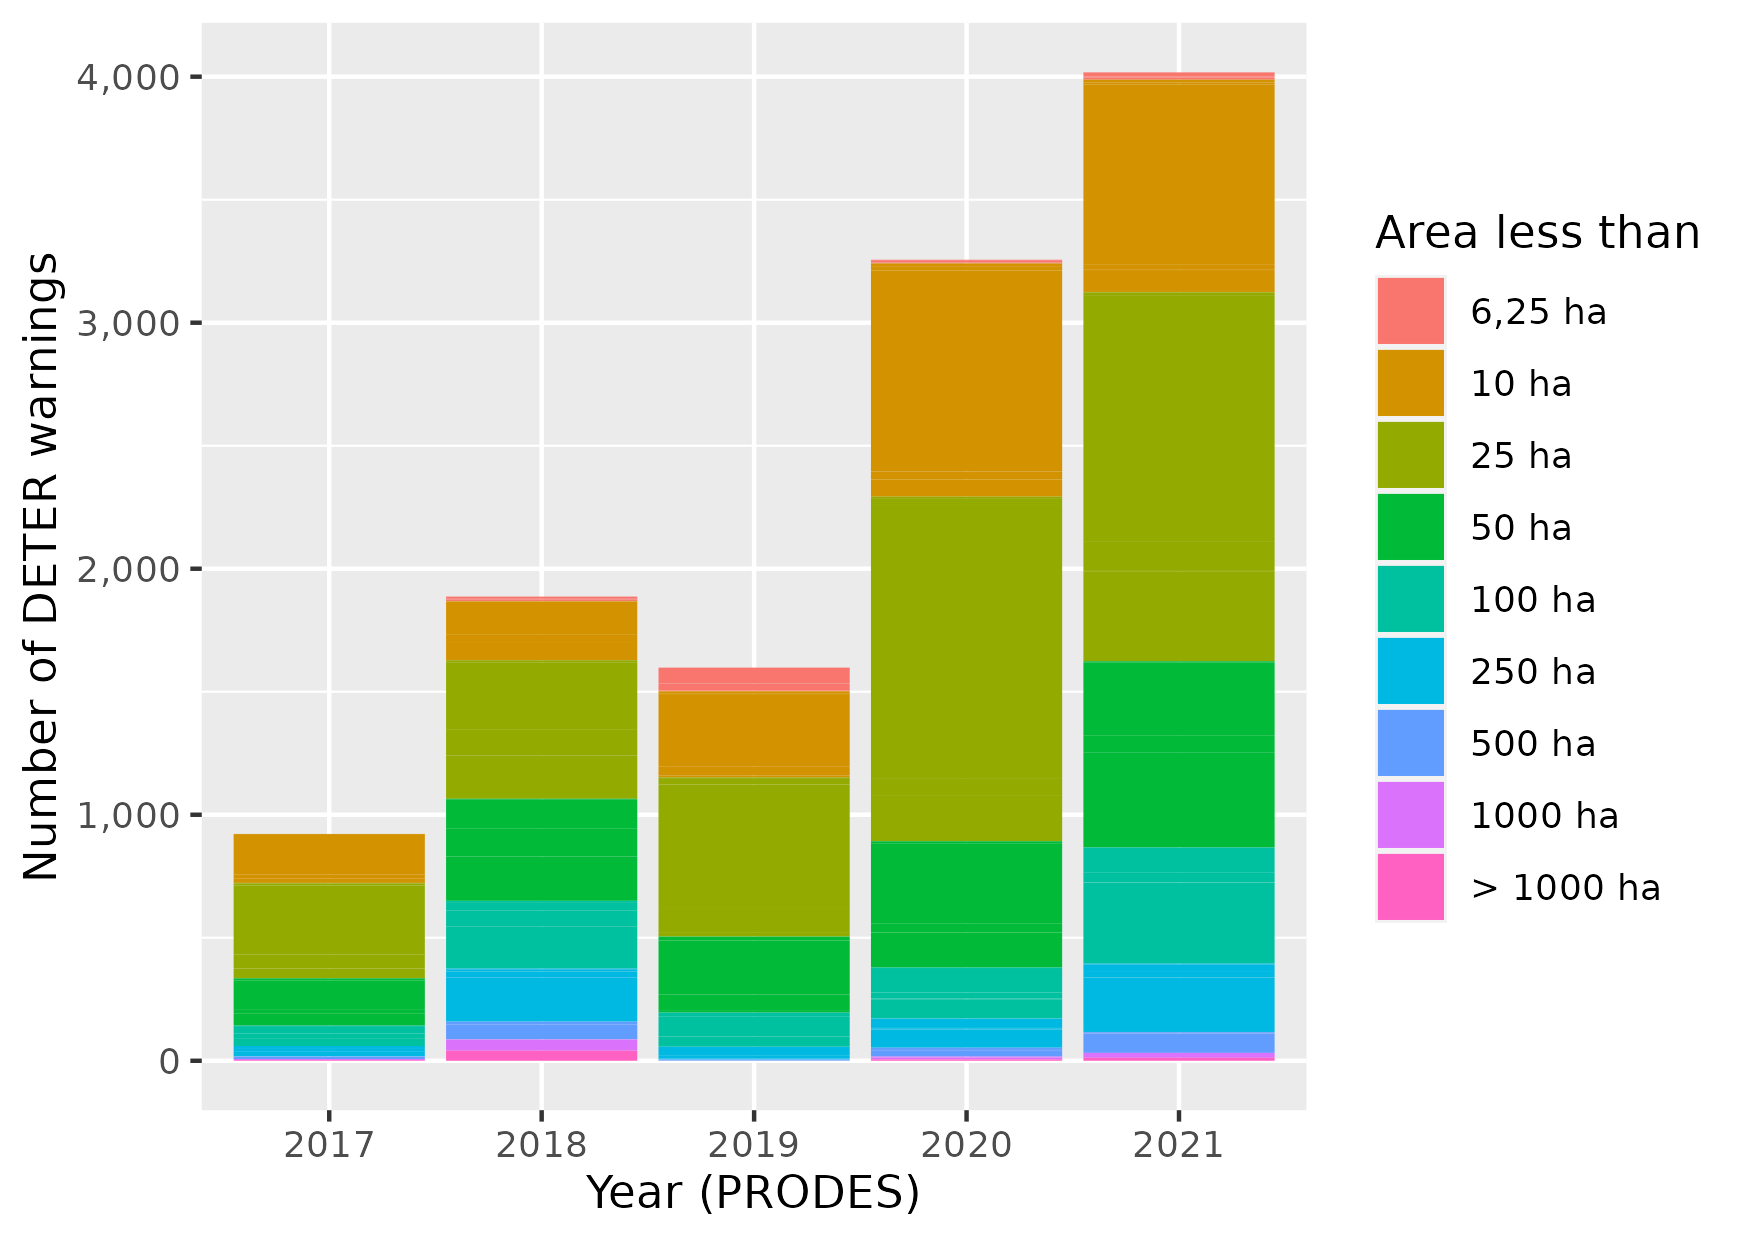
\includegraphics[width=\linewidth]{deter_warnings_size.png}
    \caption{Number of DETER alerts by year and size. Note the increasing trend
        since 2017. Note how DETER issued a similar number of alert in 2020 and
        2021 but ~Figure~\ref{fig:deter_warnings_size} shows a larger extent of
        alerts in 2021.}
    \label{fig:deter_warnings_size}
    \end{center}
\end{figure}

From August to October is when most DETER alerts are issued, and September, the peak month, presents an increasing trend in area, reaching its maximum in 2021.
This period corresponds to the fire season in most of the Brazilian Amazon~\cite{carvalho2021} (see Figure~\ref{fig:deter_warnings_size_month}). 

\begin{figure}[h] 
    \begin{center}
    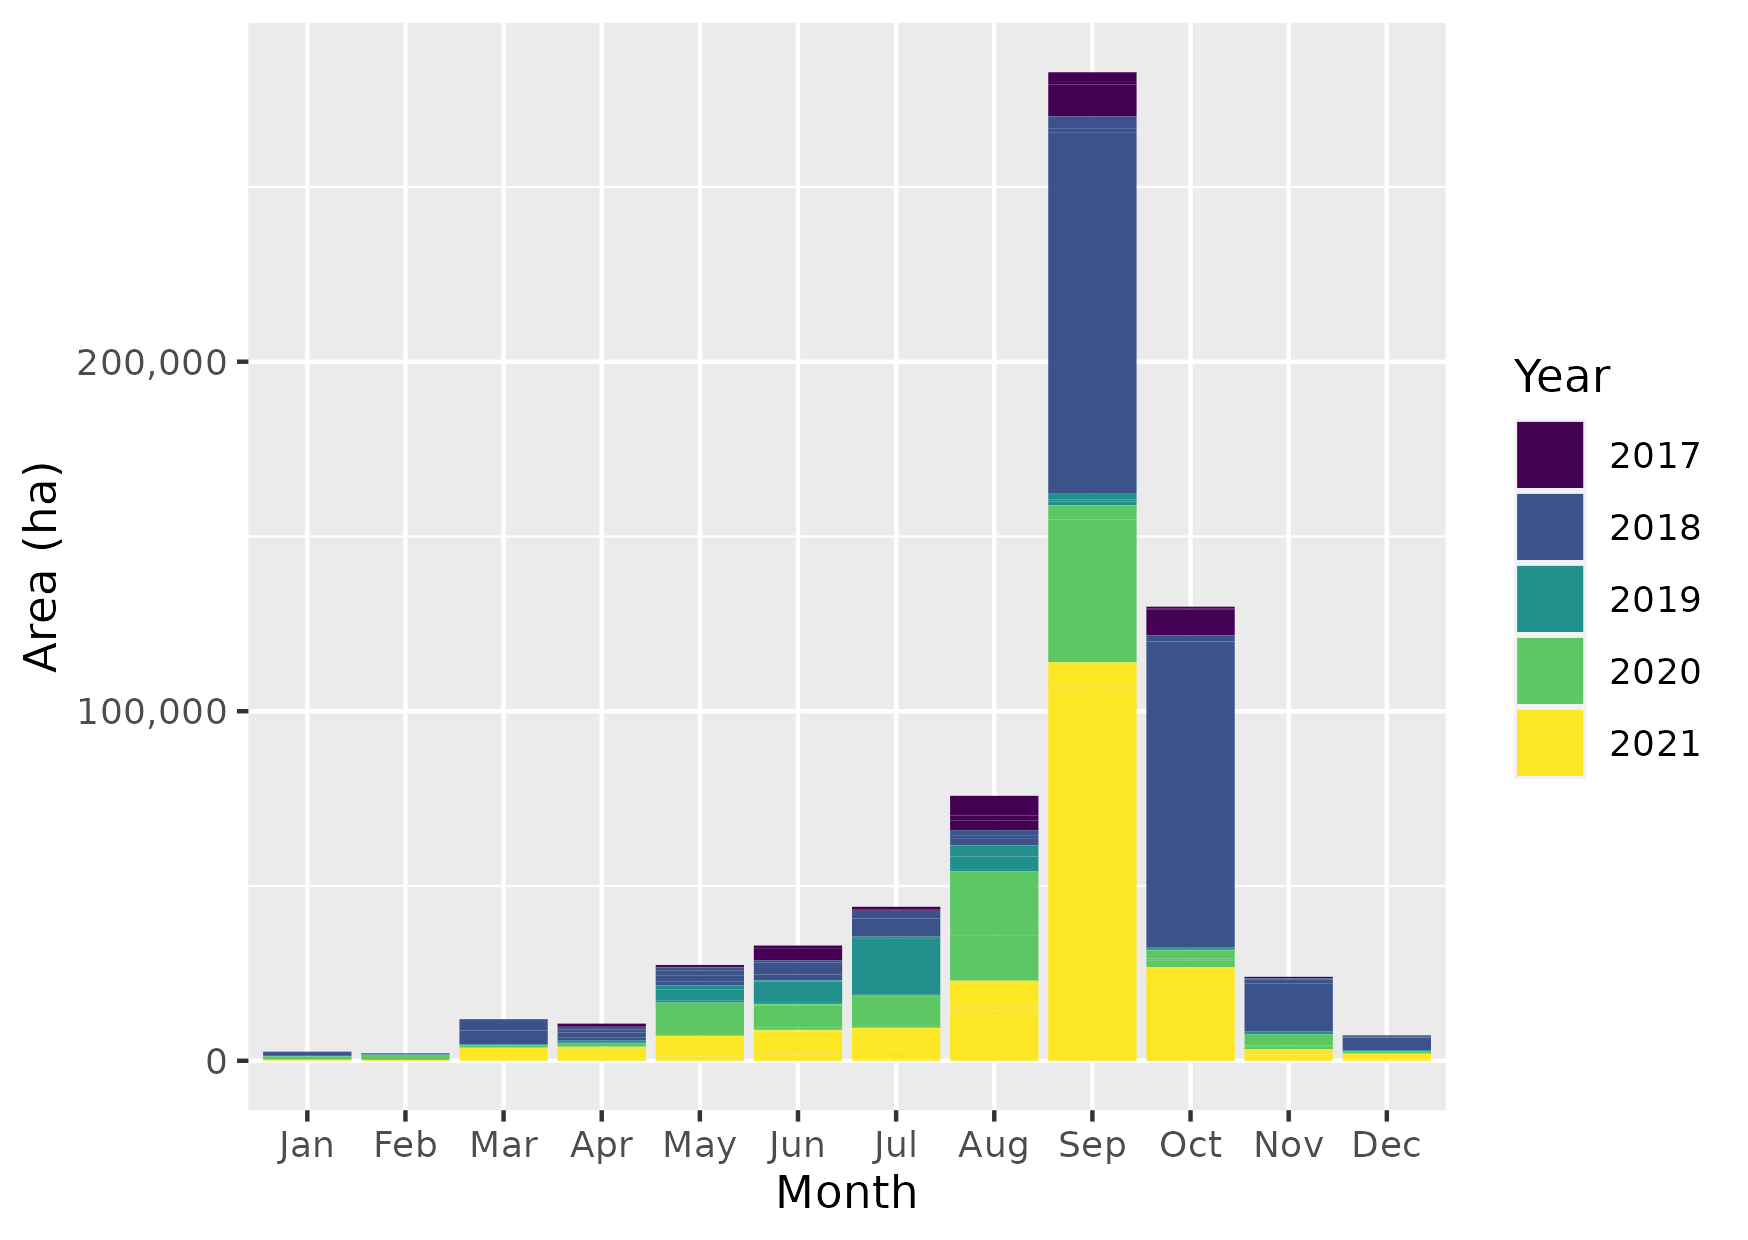
\includegraphics[width=\linewidth]{deter_warnings_size_month.png}
    \caption{DETER warnings by month. Between August and October is when most
        of the warnings are issued. Note how September presents an increasing 
        trend along the years which peaks in 2021.}
    \label{fig:deter_warnings_size_month}
    \end{center}
\end{figure}

Most DETER subareas are issued a single alert and never more than five, following an exponential decay pattern.

\begin{figure}[h] 
    \begin{center}
    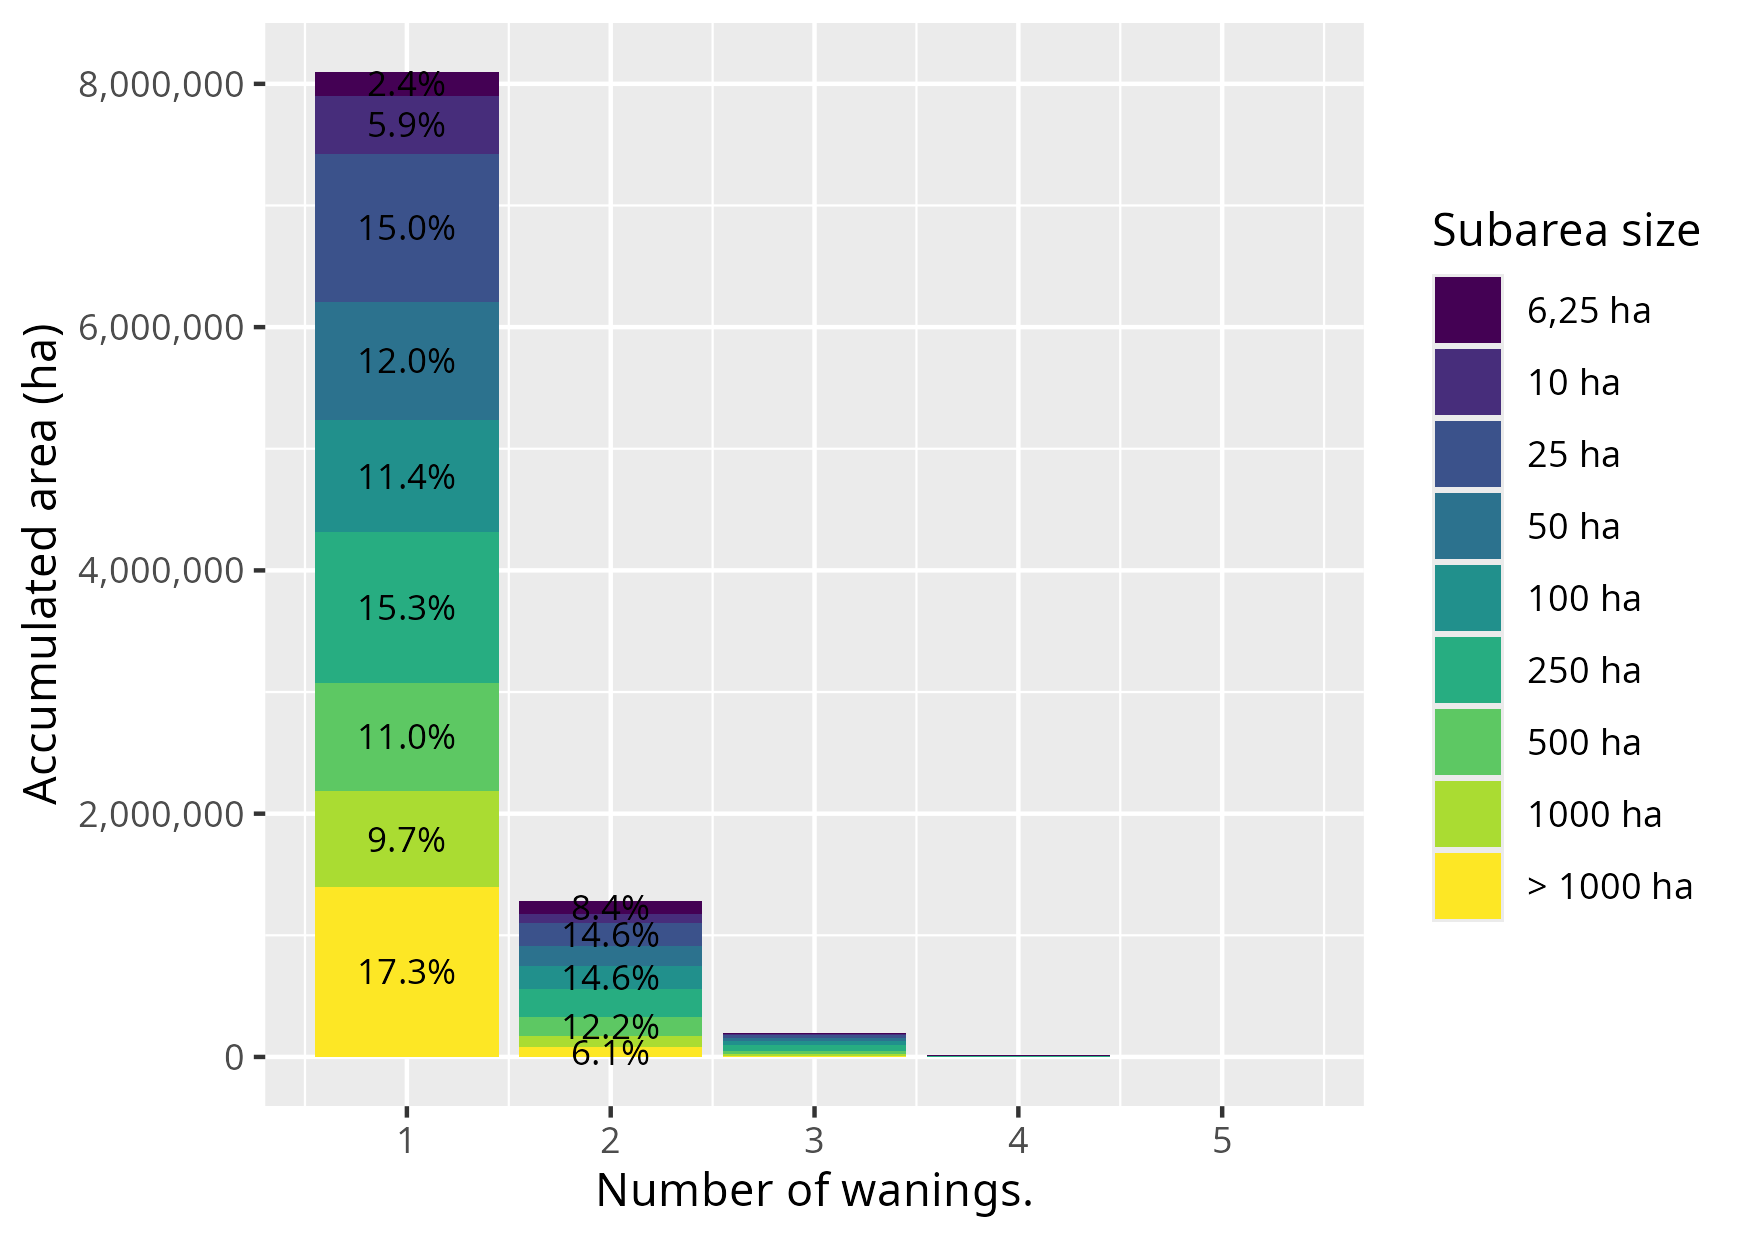
\includegraphics[width=\linewidth]{plot_area_by_warnings.png}
    \caption{DETER subareas by number of warnings. Most subareas only have one
        DETER alert and never more than five. The total extent for each number
        of alerts is homogeneously distributed.}
    \label{fig:plot_area_by_warnings}
    \end{center}
\end{figure}

%n_warnings,area_type,n_subareas,total_area_ha
1,"6,25 ha",749,3468.9305817097575
1,10 ha,2535,20277.63376261522
1,25 ha,4002,63098.2149548817
1,50 ha,1682,58496.47115551768
1,100 ha,847,58490.38486713717
1,250 ha,459,69741.03013061572
1,500 ha,133,43890.28044541861
1,1000 ha,54,36388.05024453305
1,> 1000 ha,42,108701.00171141527
2,"6,25 ha",617,2754.463872088673
2,10 ha,542,4300.325377400743
2,25 ha,829,13016.655436123781
2,50 ha,356,12588.702356866337
2,100 ha,200,14101.669591812615
2,250 ha,111,16949.55559907801
2,500 ha,25,8804.534433634506
2,1000 ha,12,8361.25238844781
2,> 1000 ha,3,6444.004258638234
3,"6,25 ha",70,331.8730328444766
3,10 ha,48,383.2278256572545
3,25 ha,62,943.440952612507
3,50 ha,15,528.551615276519
3,100 ha,5,342.0266654521489
3,250 ha,2,261.59856489548065
4,"6,25 ha",5,24.44017934602583
4,10 ha,1,8.426126639709947
4,25 ha,2,31.449280712276668


The time period between DETER alerts in the same subarea is one year, except for subareas with two alerts, when it is two years (Figure~\ref{fig:plot_days_first_to_last}). 

\begin{figure}[h] 
    \begin{center}
        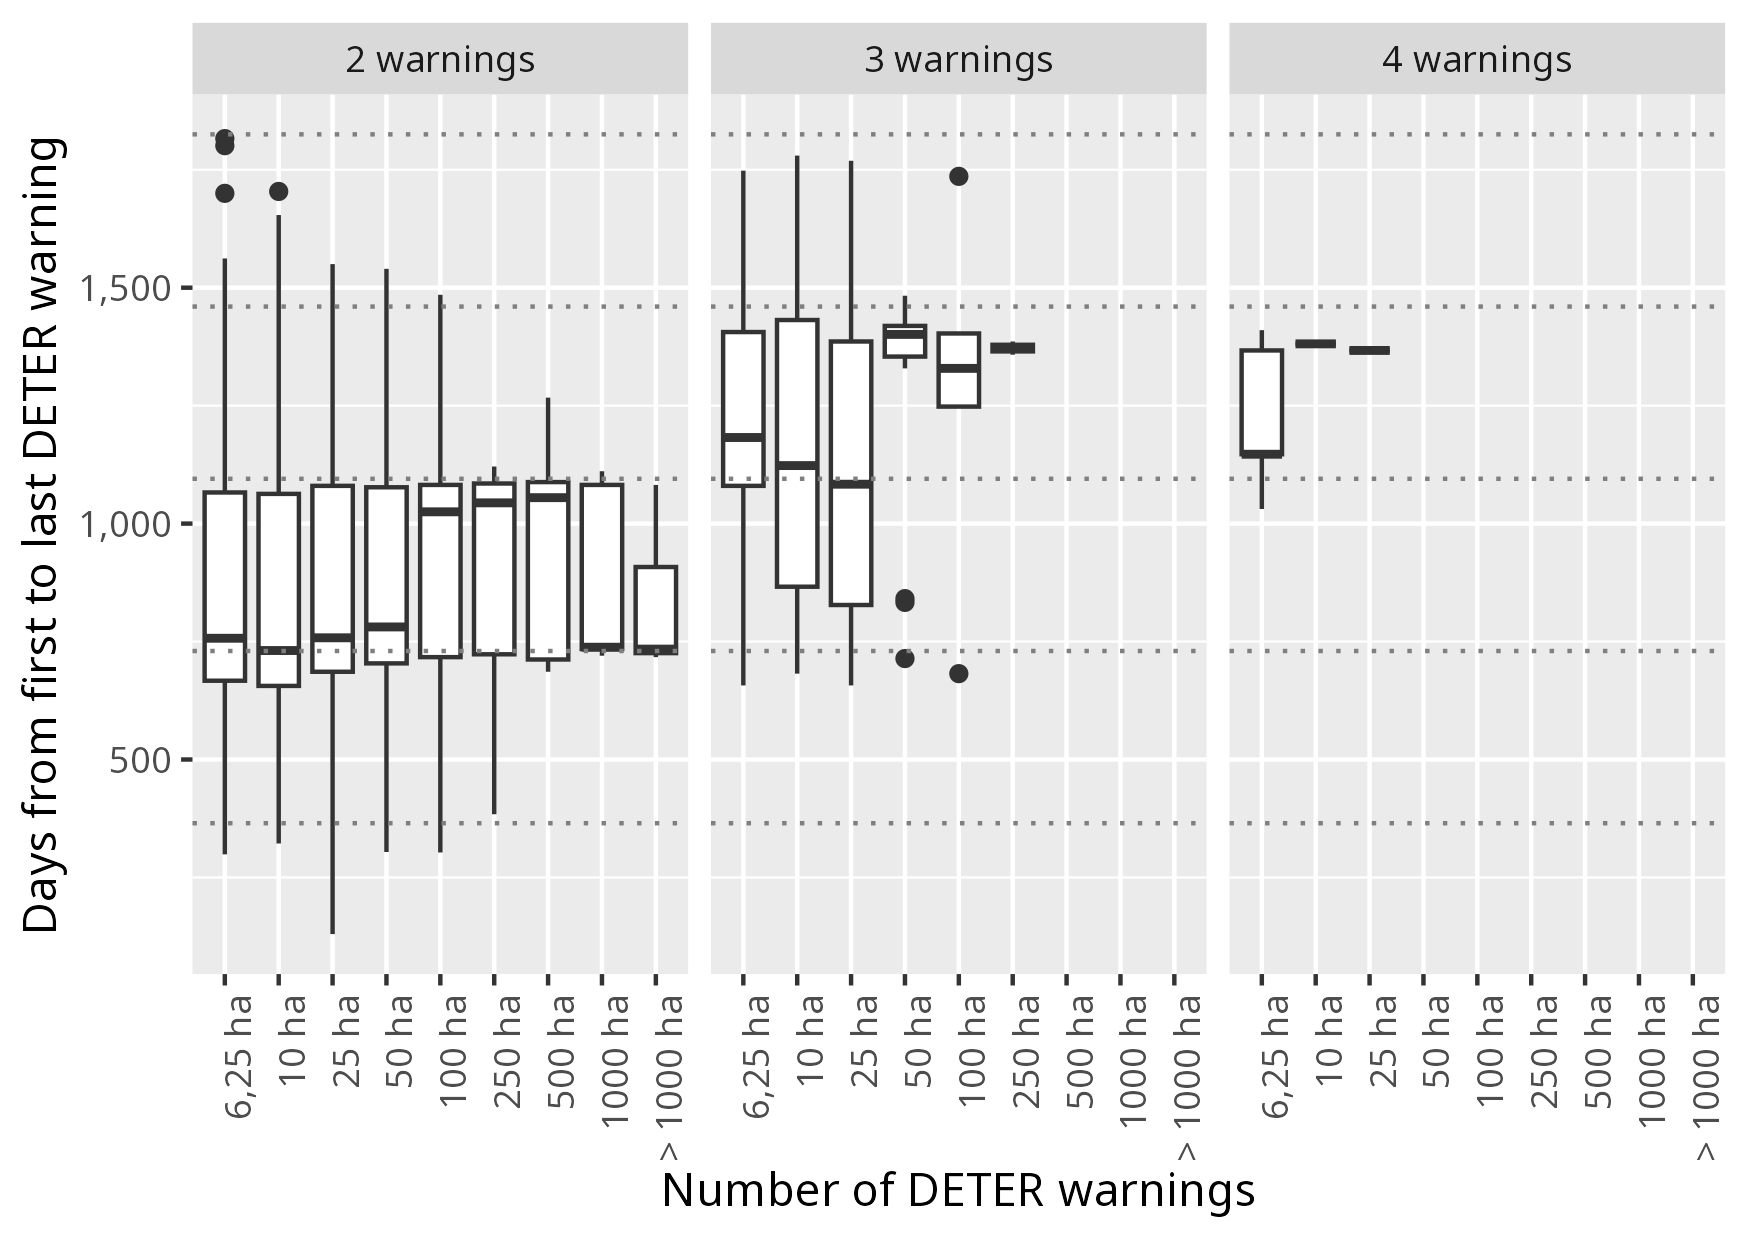
\includegraphics[width=\linewidth]{plot_days_first_to_last.png}
    \caption{Number of days between the first and last DETER alerts. The
        horizontal dashed black lines represent intervals of 365 days.
        DETER subareas with 2 warnings tend to be two years apart and then
        increase one year with each additional alert. Also note that the
        distribution by area tend to have long tails towards longer periods
        between the first and lat DETER alert.}
    \label{fig:plot_days_first_to_last}
    \end{center}
\end{figure}

The map in Figure~\ref{fig:plot_area_by_warnings} shows the distribution of recurrent deforestation warnings, that is, a surface interpolation of the number of DETER alerts.

\begin{figure}[h] 
    \begin{center}
        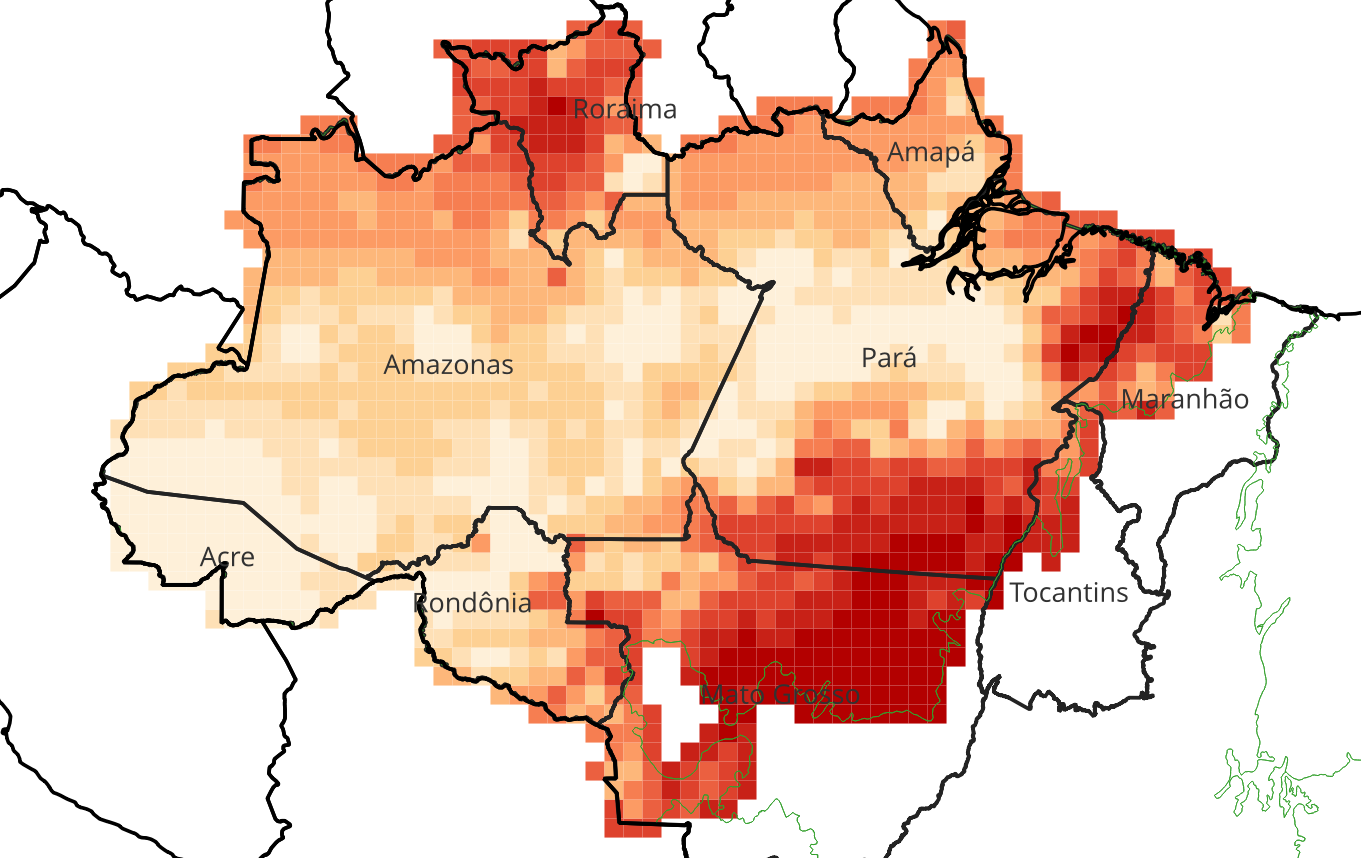
\includegraphics[width=\linewidth]{nwarnings_idw_map.png}
        \caption{Spatial distribution of recurrent degradation (number of
        alerts by subarea) in the Brazilian Amazon. Amazon's east front is
        where most of recurrent DETER alerts area found.}
    \label{fig:nwarnings_idw_map}
    \end{center}
\end{figure}

	
\section{Discussion}

Our results show that the number of subareas with more than one DETER warning
is low compared to the total number of warnings and there are but a few of 
subareas with more than three warnings.
They also show that most of successive warnings of the same subarea are at most 
four years apart, two years from the first to the second, and one year from 
there. 
We found that DETER warnings provide between two and four warnings to 
characterize degradation processes in one of the most deforested municipalities 
in the Amazon. 

The number of available subareas seems small for training Machine Learning 
algorithms, specially those based on Deep Learning that are well-known
for requiring large amounts of training data.
However, we expect these numbers increase by extending our analysis to the 
whole area covered by the Brazilian Amazon since 2016.
In addition, we think our results foster new analysis in areas different from 
Computer Science.
Despite this fact, our results are important as they explore a potential new
application of the already useful and openly available DETER data.

Our results rely on the assumption that \textit{São Félix do Xingu} is 
representative of degradation in the Amazon.
They also rely on the accuracy of DETER warning polygons and the assumption
that subareas larger than 3 ha correspond to actual degradation warnings 
instead of drawing inaccuracies on a computer screen.


	
%\section{Conclusions}

%Major headings, for example, "1. Introduction", should appear in all capital letters, bold face, centered in the column, with one blank line before, and one blank line after. Use a period (".") after the heading number, not a colon.

%If the last page of your paper is only partially filled, arrange the columns so that they are evenly balanced if possible, rather than having one long column.

%List and number all bibliographical references at the end of the paper.  The references can be numbered in order of appearance in the document.  When referring to them in the text, type the corresponding reference number in square brackets as shown at the end of this sentence \cite{Smith_year}.

%To insert citations in \LaTeX, use {\small \verb|\cite{<author>}|}, which produces ``\cite{Jones_year} ''. The bibliography is located in file {\small \verb|07_SBSR.bib|}. The references are automatically generated.

TODO.


\section{Acknowledgements}

The authors would like to acknowledge the Conselho Nacional de Desenvolvimento 
Científico e Tecnológico (CNPq Projeto: 444418/2018-0, Processo: 350820/2022-8). 
Guilherme Mataveli was financed by the São Paulo Research Foundation (FAPESP, 
grant 2019/25701-8).
Aline Pontes-Lopes was also financed by FAPESP (grant 22/04893-9).

 
%%%% Create the references below (DO NOT CHANGE) 
%%%% (MORE INFORMATION IN README.txt) %%%%

%%%%%%%%%%%%%%%%%%%%%%%%%%%%%%% ATTENTION %%%%%%%%%%%%%%%%%%%%%%%%%%%%%%%%
%%%% The file extra considerations (extra_considerations.tex) is not part of the template and must be removed from the final work. To do so, comment the line below %%%%
%\section{PAGE NUMBERING}
    
Please do \textbf{not} paginate your paper. Page numbers and conference identification will be inserted when the paper is included in the proceedings.
\pagebreak
	
\section{Illustrations, graphs, photographs and tables}
	
Illustrations must appear within the designated margins. If needed, figures may span the two columns. If possible, position illustrations at the top of columns, rather than in the middle or at the bottom. Caption and number every illustration (Figure \ref{example_figure}). The same rules apply to tables (Table \ref{example_table}). 
	
\begin{figure}[h] % use [t] here to force figure to top
    \begin{center}
    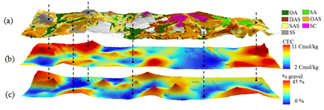
\includegraphics[width=\linewidth]{figures/example_figure.png}
    \caption{Figure caption (and also Table caption) must have a font 9 and be in bold.}
    \label{example_figure}
    \end{center}
\end{figure}

\begin{table}[h] % use [t] here to force table to top
    \centering
    \begin{tabular}{|c|c|c|c|}
        \hline
        \textbf{Item 1} & \textbf{Item 2} & \textbf{Item 3} & \textbf{Item 4}  \\
        \hline
        Value 11 & Value 12 & Value 13 & Value 14  \\
        \hline
        Value 21 & Value 22 & Value 23 & Value 24  \\
        \hline
    \end{tabular}
    \caption{Rules for table caption are the same as figures.}
    \label{example_table}
\end{table}
 

\renewcommand{\refname}{REFERENCES}
{\small
\bibliographystyle{unsrt} 
\bibliography{07_SBSR.bib}}
	
\end{document} % end of document %%%%(DO NOT CHANGE)%%%%
